\documentclass[conference]{IEEEtran}
\IEEEoverridecommandlockouts
% The preceding line is only needed to identify funding in the first footnote. If that is unneeded, please comment it out.
\usepackage{cite}
\usepackage{amsmath,amssymb,amsfonts}
\usepackage{algorithmic}
\usepackage{graphicx}
\usepackage{textcomp}
\usepackage{xcolor}
\usepackage{booktabs}
\usepackage{url}
\usepackage{cleveref}
\def\BibTeX{{\rm B\kern-.05em{\sc i\kern-.025em b}\kern-.08em
    T\kern-.1667em\lower.7ex\hbox{E}\kern-.125emX}}
\begin{document}

% NOTE: title and abstract below are suggested drafts — adjust wording to taste.
\title{Smart but Heavy or Simple but Light? Model Complexity versus Input
Resolution in Memory-Constrained Insect Crowd Counting\\
\thanks{This thesis was prepared in partial fulfilment of the requirements for the Degree of Bachelor of Computer Science, Maastricht University. Supervisor: Petra Bosilj}
}

\author{\IEEEauthorblockN{Adriane Bien}
\IEEEauthorblockA{\textit{Department of Advanced Computing Sciences} \\
\textit{Faculty of Science and Engineering}\\
\textit{Maastricht University}\\
Maastricht, The Netherlands}
}

\maketitle

\begin{abstract}
Automated monitoring of mealworm (Tenebrio molitor) rearing plates requires
counting up to hundreds of densely packed, heavily occluded larvae per image,
conditions under which density-estimation-based crowd counting is better
suited than detection. For deployment on low-cost edge hardware, peak
inference memory is the binding constraint, and it is governed by two levers:
model complexity and input resolution. This thesis asks which lever matters
more when memory is scarce, comparing a heavyweight network (CSRNet) against
a lightweight one (MobileCount) on the TenebrioVision dataset across six input
resolutions, after a per-architecture hyperparameter search at a fixed
mid-range resolution. Both networks count to within one larva of the ground
truth even when the input is downscaled to a sixteenth of the native pixel
count. CSRNet converts every further increase in resolution into accuracy,
reaching a test mean absolute error of 0.23 larvae at 1.6 GB of peak inference
memory, while MobileCount saturates near 0.36 beyond the mid resolutions,
peaking at just 204 MB. The lightweight model owns the accuracy--memory
Pareto frontier over almost the entire operating range, delivering equal or
better accuracy at six to ten times less memory; the heavyweight model is
justified only when errors below its rival's ceiling are required. Training
diagnostics indicate that this ceiling reflects optimization instability of
hyperparameters transported across resolutions rather than a proven capacity
limit.
\end{abstract}

\begin{IEEEkeywords}
crowd counting, density estimation, edge computing, model efficiency, Tenebrio molitor, precision livestock farming
\end{IEEEkeywords}

\section{Introduction}\label{sec:intro}
To meet the growing global demand for protein, insect farming has emerged as a
promising alternative to conventional livestock production~\cite{vanhuis2013}.
\textit{Tenebrio molitor}, the yellow mealworm, is one of the few insect species
approved for human consumption in Europe~\cite{eu2021tenebrio}. To be
commercially viable, however, production must scale up significantly---a challenge
that hinges directly on automation~\cite{rumpold2013}.

Automated mealworm farming requires continuous monitoring of the rearing plates
to inform decisions about feeding, harvesting, and environmental control. Prior
work has explored machine vision for this purpose, but most of it relies on
object detection and instance segmentation~\cite{majewski2022multipurpose}, which struggled with the dense,
heavily occluded scenes typical of insect rearing trays \cite{Papadopoulos2024TenebrioVision}. Crowd counting via
density estimation offers a far more suitable framework for these
conditions~\cite{Sindagi2017ASO}, yet it remains entirely unexplored in insect
agriculture.

The primary driver for automation is economic: reducing operational costs and
maximizing production efficiency~\cite{rumpold2013}. Because the industry lacks
standardization~\cite{NAWOYA2024108503}, farms have adopted a diverse range of
technological solutions~\cite{CoRoSect2022AdvancedArchitecture,
kroncke2020automation}. One compelling approach is edge AI, which is
particularly attractive for cost-sensitive operations because it runs inference
locally on low-cost embedded devices~\cite{angulo2025realtimecricketsortingsex}.
This thesis therefore investigates how crowd-counting models can be deployed
within the strict memory constraints of edge hardware, specifically the Jetson Nano.

Memory consumption during inference is governed primarily by two factors: model
complexity and input resolution. Larger architectures require more memory to
store their parameters, while higher-resolution inputs enlarge the intermediate
feature maps that must be held in memory during the forward
pass~\cite{Chao2019HarDNet}. Reducing the memory footprint therefore comes down
to two options: shrinking the model or shrinking the input.

This raises a practical question: when memory is strictly limited, is
architectural complexity or input fidelity more important? To investigate, this
thesis compares two competing strategies---deploying a ``smart but heavy'' model
that must be fed downscaled images to fit within memory, against a ``simpler but
light'' model that leaves enough headroom to process images at full resolution.

\section{Related Work}
\subsection{Crowd Counting Approaches}
Crowd counting methods can be broadly categorized into three approaches:
detection-based, regression-based, and density estimation-based methods.

The earliest approaches were detection-based, producing a population estimate by
aggregating individual bounding-box predictions. As noted above, these methods notoriously struggle under severe occlusion and high object density.

Regression-based methods were developed to address this by computing object
counts directly from image features, bypassing the need for explicit
localization. While more robust to occlusion, they sacrifice spatial information
entirely, giving no insight into how individuals are distributed across the
scene.

The most widely used crowd-counting models today are based on density
estimation. Rather than localizing individuals explicitly, this approach learns
to map an image to a density map, where the integral over any region gives the
count within it and the integral over the entire map gives the total count.
Because the map preserves where mass is concentrated across the scene, density
estimation retains the spatial information that regression discards. Models are
trained by regressing the predicted map against a ground-truth density
map~\cite{wang2020mobilecount, li2018csrnet, gao2020crowdcountingsurvey}.

\subsection{CNN-Based Density Estimation}
The success of Convolutional Neural Networks (CNNs) in image classification and
recognition has made them the de facto standard for density estimation. Rather
than relying on hand-crafted features and shallow regressors, CNNs learn
hierarchical feature representations directly from raw pixel data, enabling far
greater robustness to occlusion, lighting variation, and background
clutter~\cite{gao2020crowdcountingsurvey, li2018csrnet}.

Early approaches used basic CNNs with standard convolutional and fully connected
layers. These were simple to implement but struggled with the scale variation
inherent to crowd scenes, motivating multi-column architectures such as MCNN,
which run parallel branches with different receptive fields to capture features
at multiple scales~\cite{Zhang_2016_CVPR}.

The field has since largely shifted toward single-column designs, with CSRNet a
pivotal model in this transition. CSRNet demonstrated that a single deeper column
could outperform bloated multi-column structures through a dilated-convolution
back-end that enlarges the receptive field while preserving spatial resolution.
This design has since become one of the most widely adopted in crowd counting,
and CSRNet remains a standard baseline for benchmarking newer methods,
particularly in dense scenes~\cite{gao2020crowdcountingsurvey, li2018csrnet}.

\subsection{Lightweight Networks}
Beyond architectural design, lightweight models have emerged as a crucial area of
research for resource-constrained deployment. The objective is to minimize
computational overhead and parameter count without incurring a significant
penalty to counting accuracy~\cite{gao2020crowdcountingsurvey,
wang2020mobilecount}.

A prominent example in density-based crowd counting is MobileCount, an
encoder-decoder network built on a lightweight MobileNetV2 backbone. Compared
with CSRNet, MobileCount reduces the model footprint by roughly 80\%---only
$3.40$ million parameters versus CSRNet's $16.26$ million. As shown in
Table~\ref{tab:lit_table}, MobileCount exhibits only a minor reduction in
accuracy across standard benchmark datasets, remaining highly comparable to its
heavier counterpart. Given that it requires 52 times fewer floating-point
operations (FLOPs), this marginal trade-off in accuracy is heavily outweighed by
its gains in computational efficiency~\cite{wang2020mobilecount}.

\begin{table}[t]
    \centering
    \caption{Reported MAE for CSRNet and MobileCount on standard
    crowd-counting benchmarks. SHT: ShanghaiTech; WE: WorldExpo'10.
    ~\cite{wang2020mobilecount, li2018csrnet}}
    \label{tab:lit_table}
    \footnotesize
    \setlength{\tabcolsep}{5pt}
    \begin{tabular}{lcccc}
        \toprule
        Network     & SHT-A & SHT-B & UCF-CC-50 & WE \\
        \midrule
        CSRNet      & 68.2 & 10.6 & 266.1 & 8.6  \\
        MobileCount & 89.4 & 9.0  & 284.8 & 11.1 \\
        \bottomrule
    \end{tabular}
\end{table}

\section{Methods}
\subsection{Dataset}
This study uses the TenebrioVision dataset, developed within the CoRoSect
project. It consists of 1{,}120 high-resolution images ($3088 \times 2076$
pixels), grouped into 14 count levels of 80 images each, where every image in a
level contains a fixed number of \textit{Tenebrio molitor} larvae: 10, 15, 20,
25, 30, 35, 40, 45, 50, 60, 70, 80, 90, or 100. Each larva is labelled with a
bounding box, giving 53{,}600 annotated instances in total. TenebrioVision is
currently the only publicly available dataset reflecting the high-density
conditions typical of industrial larvae farming, making it the most suitable
benchmark for crowd-counting models in this specific
domain~\cite{Papadopoulos2024TenebrioVision}.

Following the split protocol of~\cite{Papadopoulos2024TenebrioVision}, the data
is stratified by count level: within each level the 80 images are shuffled with
a fixed random seed (42) and partitioned into 60 training, 12 validation, and 8
test images. Repeating this across all 14 levels yields 840 training, 168
validation, and 112 test images---a $75\,/\,15\,/\,10\,\%$ split in which every
count level is represented in identical proportion across all three subsets.
This stratification ensures a balanced distribution, so differences in
validation or test error cannot be attributed to one subset containing
systematically denser or sparser images.

\subsection{Models}
Two CNN-based density-estimation models are trained and evaluated: the accurate but computationally heavy CSRNet, and the lightweight, efficiency-oriented MobileCount. Together they represent complementary points on the accuracy–efficiency trade-off.

\subsubsection{CSRNet}
CSRNet's architecture consists of a front-end feature extractor and a dilated
convolutional back-end. The front-end is built from the first ten layers of a
pre-trained VGG-16 network, with the fully connected classification layers
removed. Three max-pooling operations reduce the spatial resolution to
$H/8 \times W/8$, producing a feature map that benefits from strong transfer
learning capacity while retaining meaningful spatial structure.

Rather than continuing to downsample via pooling---which would further degrade
spatial resolution and make accurate density-map reconstruction
difficult---the back-end uses dilated convolutions to expand the receptive field
without reducing resolution or adding parameters. A dilated convolution with
dilation rate $r$ effectively enlarges a $k \times k$ kernel to
$k + (k-1)(r-1)$, allowing the network to aggregate multi-scale contextual
information while keeping feature maps at a constant spatial size. CSRNet is
proposed in four configurations with varying back-end dilation rates;
configuration~B is used here, which the original paper identifies as the most
accurate and which applies a dilation rate of $2$ in every back-end layer.

A final $1 \times 1$ convolution collapses the back-end feature maps to a single
channel, producing a density map at $H/8 \times W/8$~\cite{li2018csrnet}. In the
implementation used here, this map is upsampled back to the input resolution so
that prediction and ground truth share a common grid.

\subsubsection{MobileCount}
MobileCount's encoder is based on MobileNetV2, a backbone built around an
inverted residual structure with linear bottlenecks. Each bottleneck applies a
$1 \times 1$ pointwise convolution to expand channel dimensionality, a
$3 \times 3$ depthwise convolution to capture spatial features, and a second
$1 \times 1$ pointwise convolution to project back to a lower-dimensional
representation. Separating channel mixing from spatial filtering in this way
dramatically reduces parameter count relative to standard convolutions.

To reduce computation further, MobileCount uses only four of MobileNetV2's seven
bottleneck blocks, as the original paper reports that removing the final three
improves performance alongside a substantial reduction in FLOPs. An additional
$3 \times 3$ max-pooling layer of stride 2 is inserted at the start of the
encoder, reducing input resolution early in the pipeline and cutting FLOPs by
over 70\% at marginal accuracy cost. Together with the initial stride-2
convolution, this reduces the resolution at the first bottleneck block to
$H/4 \times W/4$; subsequent blocks downsample further to $H/8$, $H/16$, and
$H/32$.

The decoder is a simplified LightWeight RefineNet, originally developed for
real-time semantic segmentation. It progressively fuses the four multi-scale
encoder feature maps through a series of Chained Residual Pooling (CRP) and
fusion blocks, upsampling from $H/32$ back through each scale until reaching
$H/4$. A final $3 \times 3$ convolutional layer maps this representation to a
single-channel output at $H/4 \times W/4$, which is then bilinearly upsampled
$4\times$ to full input resolution to produce the predicted density
map~\cite{wang2020mobilecount}.

\subsection{Loss Function}
Both models are trained end-to-end using the mean squared error loss between the predicted density map $D^{PM}$ and the ground truth density map $D^{GT}$:

\begin{equation}
    \mathcal{L} = \frac{1}{N} \sum_{i=1}^{N} \| D^{PM}(i) - D^{GT}(i) \|_2^2
\end{equation}

where $N$ is the number of training samples. The final population estimate is obtained by integrating the predicted density map over the full image. \cite{wang2020mobilecount, li2018csrnet}

\subsection{Image Resolution}
To investigate the impact of input scale on counting performance, both models are evaluated across a hierarchy of six resolutions. These are derived by progressively halving the original $3088 \times 2076$ images (rounding up on odd dimensions), giving: $1544 \times 1038$, $772 \times 519$, $386 \times 260$, $193 \times 130$, $97 \times 65$, and $49 \times 33$.

\subsection{Ground Truth Generation}
Point annotations are derived from the centre of each bounding box to construct
a discrete point map. Ground-truth density maps are then generated by convolving
this point map with a Gaussian kernel. Formally, for a set of $N$ annotated
positions, the density map $D(\mathbf{x})$ is defined as
\begin{equation}
    D(\mathbf{x}) = \sum_{i=1}^{N} \delta(\mathbf{x} - \mathbf{x}_i) *
    G_{\sigma}(\mathbf{x}),
\end{equation}
where $\delta(\mathbf{x} - \mathbf{x}_i)$ is a Dirac delta centred at larva
position $\mathbf{x}_i$ and $G_{\sigma}$ is an isotropic Gaussian kernel with
standard deviation $\sigma$.

A fixed-sigma kernel was applied to every annotation, following the strategy
CSRNet uses on ShanghaiTech Part~B. That dataset's structural
characteristics---a fixed viewpoint, roughly constant object size, and
comparatively uniform density---closely mirror those of TenebrioVision, and
CSRNet models it with a fixed kernel of $\sigma = 15$, approximately half the
typical head diameter. The same object-to-kernel ratio is adopted here: the standard
deviation is set to $\sigma = \texttt{bbox}/2$, where \texttt{bbox} is the
average larva bounding-box size in TenebrioVision, so that $\sigma$ again spans
roughly half the object's diameter.
% FIXME (fact-check): the sigma actually used (24 px at 1544x1038, i.e. 48 px at
% full resolution) implies an object size of 96 px, but the mean bbox side in the
% annotations is ~169 px (min side 119, sqrt-area 157). The realised ratio is
% closer to bbox/3.5 than bbox/2. Either re-derive the number you used for
% "average bbox size" or reword this justification. See fact-check report.

The kernel was truncated to an effective window of $8\sigma + 1$ pixels. To
preserve the relative spatial extent of the density distribution across scales,
$\sigma$ was scaled proportionally with resolution, giving values of 24, 12, 6,
3, 2, and 1 pixels for the six variants respectively (rounded to the nearest
pixel at the two smallest scales).

\subsection{Evaluation Metrics}\label{sec:eval_metrics}
Following standard practice in the crowd-counting literature~\cite{gao2020crowdcountingsurvey}, Mean Absolute Error (MAE) and Mean Squared Error (MSE) are used as the primary accuracy metrics:

\begin{equation}
    \text{MAE} = \frac{1}{N} \sum_{i=1}^{N} \left| y_i - \hat{y}_i \right|,
\end{equation}
\begin{equation}
    \text{MSE} = \sqrt{\frac{1}{N} \sum_{i=1}^{N}
    \left( y_i - \hat{y}_i \right)^2},
\end{equation}
where $N$ is the number of test images, $y_i$ is the ground-truth count, and
$\hat{y}_i$ is the predicted count. MAE reflects the average magnitude of
prediction error, while MSE penalises larger errors more heavily, making it
sensitive to outliers.

\paragraph{Hardware and memory measurement}
All training, evaluation, and measurements were performed in PyTorch on an
NVIDIA GeForce RTX 5070 Ti with 16\,GB of VRAM. Peak inference memory is
measured per network and resolution as the CUDA allocator's high-water mark
during a batch-1 forward pass after warm-up, and covers the resident weights,
the input, and the peak activations together; the checkpoint buffer is released
after loading, so weights are counted once. Reported values are allocated
peaks; the allocator's reserved pool is somewhat higher. Because the memory
footprint of a convolutional forward pass depends only on the input dimensions,
not on its content, the numbers hold for any input at a given resolution.

\subsection{Experimental Design}
A model's hyperparameter configuration has a substantial effect on its final
accuracy. A fair comparison between architectures must therefore evaluate each in
a setting appropriate to it, rather than imposing a single shared configuration
that may favour one design over the other.

The original CSRNet implementation was optimised with Stochastic Gradient
Descent (SGD) at a fixed learning rate of $1\times10^{-6}$ and a batch size of
$1$~\cite{li2018csrnet}. Subsequent work,
however, reports that the Adam optimiser yields faster convergence and stronger
final performance for this architecture even when all other original parameters
are held constant~\cite{jimaging7020021}. The original MobileCount implementation
used Adam with an initial learning rate of $1\times10^{-4}$, an exponential
learning-rate decay of $0.995$ per epoch, a weight decay of $1\times10^{-4}$, and
a batch size of $6$~\cite{wang2020mobilecount}.

All experiments are implemented in the C\textsuperscript{3}
Framework~\cite{gao2019c3}, a widely used crowd-counting codebase whose authors
have already tuned the supported architectures on the standard benchmark
datasets; these configurations define the starting point for tuning
(Table~\ref{tab:baseline_hyperparameters}). The configurations for the ShanghaiTech~Part~B dataset were adopted here.

\begin{table}[t]
    \centering
    \caption{Baseline (pre-tuning) optimisation hyperparameters.}
    \label{tab:baseline_hyperparameters}
    \begin{tabular}{lcc}
        \toprule
        Hyperparameter & CSRNet & MobileCount \\
        \midrule
        Optimiser             & \multicolumn{2}{c}{Adam} \\
        Weight decay          & \multicolumn{2}{c}{$1\times10^{-4}$} \\
        Batch size            & \multicolumn{2}{c}{$6$} \\
        Initial learning rate & $1\times10^{-5}$ & $1\times10^{-4}$ \\
        LR decay (per epoch)  & \multicolumn{2}{c}{step $\gamma=0.995$} \\
        \bottomrule
    \end{tabular}
\end{table}


\subsubsection{Fixed Design Decisions}
Before any hyperparameter was swept, several decisions were frozen so that every configuration was compared on equal terms: the weight decay, the training budget and learning-rate decay, the density-target scaling, and the choice of tuning resolution.

\paragraph{Weight decay.}
Both architectures use the C\textsuperscript{3} framework's default weight decay of $1\times10^{-4}$ (\cref{tab:baseline_hyperparameters}). No preliminary
testing suggested that this value was problematic, and since weight decay interacts with both the learning rate and the optimiser, tuning it jointly with them would have made the sweep infeasibly large.

\paragraph{Training budget and learning-rate decay.}
Both architectures use a fixed budget of $1500$ epochs with no early stopping, giving every configuration equal compute. With the framework's step decay of $\gamma=0.995$ per epoch, the learning rate is reduced to $0.995^{1500}\approx0.05\%$ of its base value by the end
of training. Because the decay is relative, the same epoch count is valid for every base learning rate.

\paragraph{Density-target scaling.}
The framework multiplies the density-map regression target by a
constant scaling factor $k$ (\texttt{LOG\_PARA} in the framework's
terminology) and divides the prediction by $k$ at evaluation time, so
that the per-pixel targets are of a magnitude the network can regress
comfortably. The values validated in the original works were taken as the starting point:
$k=100$ for CSRNet and $k=2550$ for MobileCount, both established on
ShanghaiTech~Part~B. Since a density map sums to the object count, its
per-pixel magnitude is inversely proportional to the number of pixels;
a value of $k$ tuned at one resolution is therefore wrong at every
other. The original values were consequently anchored to the resolution
variant closest in pixel count to ShanghaiTech~Part~B, namely
$772\times519$, and scaled in proportion to pixel count for all other variants,
\begin{equation}
    k(r) \;=\; k_{\mathrm{base}}\cdot
    \frac{A(r)}{A(772\times519)},
    \label{eq:logpara_scaling}
\end{equation}
where $A(\cdot)$ denotes the number of pixels.

\paragraph{Choice of tuning resolution.}
All tuning was performed on the $386\times260$ variant, the mid-range point of the six resolution variants spanning $49\times33$ to $1544\times1038$. The smaller the variant, the more image detail is lost and the less meaningful the resulting hyperparameter signal; the larger the variant, the slower the sweep (an estimated ${\approx}26$\,h per CSRNet run at the top resolution). The $386\times260$ variant is thus the cheapest \emph{healthy} regime: a full training run takes ${\approx}1$\,h for MobileCount and ${\approx}2.7$\,h for CSRNet, so dozens of configurations can be swept. Being mid-range, the selected hyperparameters must extrapolate in both directions; they are frozen after tuning and reused across all six resolutions to permit a fair cross-resolution comparison.

\subsubsection{Hyperparameter Tuning Protocol}
Four axes were tuned: the augmentation scheme, the optimiser, the base learning rate, and the batch size. The augmentation scheme was settled first and frozen for all subsequent experiments. Optimiser and learning rate were then swept jointly as a full grid, as preliminary
testing showed the two to be too tightly coupled to tune
independently. Batch size was swept last, around the resulting optimum, with the learning rate scaled by the standard $\sqrt{B/6}$
rule rather than as a full grid, which would have been prohibitively
expensive. All runs use a fixed random seed ($3035$). Throughout,
validation MAE is computed after every epoch and the checkpoint with
the lowest validation MAE is selected. As a sanity criterion for the
fixed $1500$-epoch budget, a run whose best checkpoint lands in the
final ${\sim}5\%$ of epochs would indicate an insufficient budget;
this did not occur for any competitive configuration.

\paragraph{Augmentation.}
With only $840$ training images, patch-based augmentation is standard
practice in crowd counting, and the two reference implementations each
prescribe a scheme. MobileCount samples a random crop spanning $80\%$
of the image online, drawn afresh at every iteration~\cite{wang2020mobilecount}. CSRNet instead expands the dataset offline into $18$ fixed patches per image: four non-overlapping quarters and five random quarter-size crops, each duplicated by horizontal mirroring~\cite{li2018csrnet}. The two schemes therefore differ not only in when patches are drawn but also in patch size and mirroring; they are compared here as complete recipes rather than factor by factor. Both schemes were trained at $386\times260$ under the baseline hyperparameters, and their best-validation checkpoints were additionally scored on the training split to expose any memorisation gap (Table~\ref{tab:aug_paper_schemes}).

\begin{table}[t]
    \centering
    \caption{Augmentation schemes at $386\times260$ under the baseline
    hyperparameters: MAE of the best-validation checkpoint on the train
    and validation splits, and the generalisation gap
    $\Delta = \text{val} - \text{train}$.}
    \label{tab:aug_paper_schemes}
    \small
    \begin{tabular}{l rrrrrr}
        \toprule
        & \multicolumn{3}{c}{CSRNet}& \multicolumn{3}{c}{MobileCount}\\

        Scheme& train & val & $\Delta$ & train & val & $\Delta$ \\
        \midrule
        $80\%$ crop& $3.465$ & $3.513$ & $+0.05$ & $0.621$ & $0.632$ & $+0.011$ \\
        $18$-patch& $4.085$ & $4.074$ & $-0.01$ & $0.640$ & $0.622$ & $-0.018$ \\
        \bottomrule
    \end{tabular}
\end{table}

Neither scheme overfits under this training budget: train and validation
error remain essentially identical in all four runs, so on the
generalisation criterion the comparison is a tie. (CSRNet's high absolute
errors here reflect the untuned Adam baseline; they fall by an order of
magnitude after tuning, cf.\ Table~\ref{tab:lr_grid}.)

The online crop was adopted for both architectures. It was at least as accurate in these runs, and it is the cheaper and simpler choice: the offline scheme would have to precompute $90{,}720$ patch--density-map pairs across the six variants, whereas the online crop adds
only a random slice per iteration. It also exposes the network to an
effectively unbounded set of distinct crops rather than a fixed pool,
and has become the prevailing pattern in modern crowd-counting
pipelines.

Because the crop is defined as a fraction of the image rather than in
absolute pixels, the scheme transfers unchanged across all resolution
variants. Validation and test images are always processed whole.

\paragraph{Optimiser and learning rate.}
Table~\ref{tab:lr_grid} presents the joint optimiser~$\times$~learning-rate grid. The compared optimisers, Adam and AdamW, differ only in how the (fixed) weight decay enters the update — Adam folds it into the
gradient before the adaptive normalisation, whereas AdamW applies it
as a separate, decoupled term.

The learning rate was swept in decades spanning one decade below and one above each network's framework optimum
(Table~\ref{tab:baseline_hyperparameters}). Because the best cell
landed on the upper edge for both networks, the sweep was extended by
one further decade ($10^{-3}$ for CSRNet, $10^{-2}$ for MobileCount).

Both extension runs diverged, under either optimiser. Under AdamW, CSRNet at
$10^{-3}$ never escaped a constant-output regime: its best validation MAE of
$22.85$, reached at epoch $2$, coincides with the best achievable constant
prediction (predicting the dataset median count for every image yields MAE
$22.9$; predicting the mean, $23.3$), after which the error settles permanently
at $27.7$. MobileCount at $10^{-2}$ briefly reached MAE $1.50$ within the first
$25$ epochs before destabilising and settling at $26.6$. Both runs therefore end
noticeably \emph{worse} than a trivial constant predictor and are omitted from
Table~\ref{tab:lr_grid}.

Two regularities emerge from the grid. First, each architecture has its own optimal learning rate, exactly one decade apart: $10^{-4}$ for CSRNet and $10^{-3}$ for MobileCount, in both cases one decade above
the framework default.

Second, at its optimal learning rate, each network prefers
AdamW, but by margins that differ by an order of magnitude: for
CSRNet the gap is dramatic ($0.320$ vs.\ Adam's best of $2.74$ at any
learning rate), while for MobileCount it is modest ($0.385$ vs.\
$0.420$). CSRNet's ImageNet-pretrained, batch-norm-free VGG-16 frontend is progressively eroded by Adam's coupled weight decay, which is amplified by the adaptive normalisation wherever gradients are small, leaving Adam uncompetitive at every learning rate. MobileCount, which is batch-normalised and trained from
scratch — and therefore largely invariant to the scale of its weights
— tolerates coupled decay far better, and Adam trails AdamW only modestly.
The training curves also reveal a behavioural difference: CSRNet's validation MAE descends to a plateau and remains there, so its final and best checkpoints nearly coincide, whereas MobileCount reaches its
optimum mid-training and drifts mildly upward thereafter — most
visibly at $10^{-4}$ — so checkpoint selection matters for its
reported accuracy.

\begin{table}[t]
    \centering
    \caption{Best validation MAE over the optimiser $\times$
    learning-rate grid ($386\times260$, batch size $6$, $1500$ epochs).
    Asterisks mark the framework defaults.}
    \label{tab:lr_grid}
    \begin{tabular}{ccc@{\hspace{2em}}ccc}
        \toprule
        \multicolumn{3}{c}{CSRNet} & \multicolumn{3}{c}{MobileCount} \\
        \midrule
        LR & Adam* & AdamW & LR & Adam* & AdamW \\
        $10^{-6}$  & $2.74$ & $0.923$          & $10^{-5}$  & $0.880$ & $0.831$ \\
        $10^{-5}$* & $3.51$ & $0.394$          & $10^{-4}$* & $0.632$ & $0.542$ \\
        $10^{-4}$  & $4.33$ & $\mathbf{0.320}$ & $10^{-3}$  & $0.420$ & $\mathbf{0.385}$ \\
        \bottomrule
    \end{tabular}
\end{table}

\paragraph{Batch size.}
After fixing the optimiser and learning rate, batch size was tuned. Because the optimal learning rate scales with batch size, each batch size $B\in\{1,2,4,8\}$ was evaluated at its own $\sqrt{B/6}$-scaled learning rate, anchored to each network's batch-size-$6$ optimum; this keeps the scale of the per-step gradient noise approximately constant, so the sweep isolates the batch-size effect rather than conflating it with an untuned learning rate.

The result (Table~\ref{tab:batchsize}) is a clean divergence: CSRNet prefers small batches; MobileCount prefers large ones.
For CSRNet, MAE improves steadily as the batch shrinks, with the
benefit concentrated below batch size $4$; batch size $1$ ($0.288$) is
the best result obtained at this resolution. MobileCount's optimum
sits at the batch-size-$6$ anchor ($0.385$), with batch sizes $4$ and
$8$ close behind, while batch size $1$ collapses to MAE $2.85$. The
dominant cause is architectural: MobileCount's batch-normalisation
statistics degenerate when each batch contains a single sample.
CSRNet, whose VGG-16 frontend contains no batch normalisation, is
immune to this failure mode — consistent with the reference
implementation's choice of batch size $1$~\cite{li2018csrnet}.

\begin{table}[h]
\centering
\caption{Batch-size sweep at $\sqrt{B/6}$-scaled learning rates (AdamW,
$386\times260$, $1500$ epochs; best validation MAE). The batch-size-$6$
rows are the anchor cells from Table~\ref{tab:lr_grid}; best per
network in bold.}
\label{tab:batchsize}
\begin{tabular}{l cc@{\hspace{2em}}cc}
\toprule
 & \multicolumn{2}{c}{CSRNet} & \multicolumn{2}{c}{MobileCount} \\
Batch size& LR & MAE & LR & MAE \\
\midrule
$1$   & $4.0\times10^{-5}$ & $\mathbf{0.288}$ & $4.0\times10^{-4}$ & $2.85$ \\
$2$   & $6.0\times10^{-5}$ & $0.292$          & $6.0\times10^{-4}$ & $0.543$ \\
$4$   & $8.0\times10^{-5}$ & $0.307$          & $8.0\times10^{-4}$ & $0.436$ \\
$6$*  & $1.0\times10^{-4}$ & $0.320$          & $1.0\times10^{-3}$ & $\mathbf{0.385}$ \\
$8$   & $1.2\times10^{-4}$ & $0.319$          & $1.2\times10^{-3}$ & $0.460$ \\
\bottomrule
\end{tabular}
\end{table}


\subsubsection{Final Selected Configurations}
\label{subsec:final_configs}

The selected configurations for both networks are summarised in
Table~\ref{tab:final_configs}. Relative to the framework baselines
trained under the identical protocol (the asterisked cells of
Table~\ref{tab:lr_grid}), tuning improves the best validation MAE from
$3.51$ to $0.288$ for CSRNet and from $0.632$ to $0.385$ for
MobileCount. Notably, both networks end up on the same optimiser but
retain an architecture-specific learning rate and batch size — neither network's optimum would have been found by tuning on the other
and transferring.

\begin{table}[h]
    \centering
    \caption{Final selected configurations.}
    \label{tab:final_configs}
    \begin{tabular}{lcc}
        \toprule
        & CSRNet & MobileCount \\
        \midrule
        Optimiser             & \multicolumn{2}{c}{AdamW} \\
        Initial learning rate & $4\times10^{-5}$ & $1\times10^{-3}$ \\
        Batch size            & $1$ & $6$ \\
        Weight decay          & \multicolumn{2}{c}{$1\times10^{-4}$} \\
        LR schedule           & \multicolumn{2}{c}{step $\gamma=0.995$} \\
        Training budget       & \multicolumn{2}{c}{$1500$ epochs} \\
        Augmentation          & \multicolumn{2}{c}{online $80\%$ crop} \\
        Density-target scale $k$ & $100$ & $2550$ \\
        & \multicolumn{2}{c}{\footnotesize scaled per Eq.~\eqref{eq:logpara_scaling}} \\
        Random seed           & \multicolumn{2}{c}{$3035$} \\
        \bottomrule
    \end{tabular}
\end{table}

\section{Results}\label{sec:results}
The tuned configurations (Table~\ref{tab:final_configs}) were retrained from
scratch at each of the six resolution variants. Table~\ref{tab:resolution_test}
reports, for every network~$\times$~resolution cell, the error of the
best-validation-MAE checkpoint on all three splits; each checkpoint is
evaluated exactly once on the test split.

\begin{table*}[t]
    \centering
    \caption{Counting error across input resolutions, in larvae per
    image (metrics as defined in Section~\ref{sec:eval_metrics}). Each
    cell's best-validation-MAE checkpoint is evaluated exactly once on
    the test split ($112$ images). The asterisk marks the tuning
    resolution; bold marks the best value per column. MobileCount's
    test differences across the three largest resolutions are within
    run-to-run noise (see text).}
    \label{tab:resolution_test}
    \small
    \begin{tabular}{l lrrr lrrr}
        \toprule
        & \multicolumn{4}{c}{CSRNet}& \multicolumn{4}{c}{MobileCount}\\

              Resolution&  train MAE&val MAE & test MAE & test MSE &  train MAE&val MAE & test MAE & test MSE \\
        \midrule
        $49\times33$     &  5.94&$5.96$  & $5.46$  & $6.22$  &  2.61&$2.68$  & $2.92$  & $3.96$ \\
        $97\times65$     &  0.81&$1.03$  & $1.36$  & $2.40$  &  2.06&$1.91$  & $2.00$  & $2.95$ \\
        $193\times130$   &  0.29&$0.534$ & $0.885$ & $1.83$  &  0.86&$0.861$ & $0.895$ & $1.25$ \\
        $386\times260^*$ &  0.16&$0.288$ & $0.470$ & $0.973$ &  0.40&$\mathbf{0.385}$ & $0.433$ & $0.653$ \\
        $772\times519$   &  0.08&$0.193$ & $0.289$ & $0.683$ &  0.44&$0.434$ & $0.471$ & $0.618$ \\
        $1544\times1038$ &  0.09&$\mathbf{0.183}$ & $\mathbf{0.233}$ & $\mathbf{0.479}$ &  0.33&$0.428$ & $\mathbf{0.361}$ & $\mathbf{0.521}$ \\
        \bottomrule
    \end{tabular}
\end{table*}

\subsection{Accuracy Across Resolutions}
Both architectures tolerate substantial downscaling well. The test MAE stays
below one larva down to a resolution of $193\times130$, meaning that halving
the input twice from the tuning anchor costs very little in absolute counting
accuracy. Below $193\times130$, however, performance degrades sharply. At the
lowest resolution ($49\times33$) both networks are heavily compromised:
CSRNet's test MAE rises to $5.46$ — a $23\times$ increase over its best result
— while MobileCount degrades more gracefully to $2.92$.

Measured against the dataset's mean count of $47.9$ larvae per image, the
best-performing models ($1544\times1038$) count to within roughly $0.5$ to
$0.75\%$ of the ground truth, whereas the lowest-resolution variants
($49\times33$) deviate by $6$ to $11\%$. The MSE columns follow the same
pattern throughout, so these conclusions are not an artefact of the choice of
error metric.

Despite these similarities under downscaling, the two models behave entirely
differently when scaling up. CSRNet scales monotonically: its test MAE
decreases with every resolution step, reaching $0.233$ at
$1544\times1038$ — the strongest overall result obtained in this thesis.
CSRNet consistently converts additional spatial information into counting
accuracy.

MobileCount, by contrast, scales non-monotonically. Selected by validation
MAE, the network favours its tuning resolution ($0.385$), and further
upscaling yields no validation gains ($0.434$ at $772\times519$, $0.428$ at
$1544\times1038$). Its best test-split performance nevertheless lands at the
highest resolution ($0.361$), so validation and test disagree on the optimal
setting. Because its three largest-resolution results fluctuate between
$0.36$ and $0.47$ with no consistent ordering, these differences are best read
as run-to-run optimisation noise. In practice, MobileCount reaches an accuracy
ceiling around MAE $0.4$ and cannot reliably translate higher input resolution
into better accuracy.

\subsection{Training Dynamics}
The learning curves (Figure~\ref{fig:res_learning_curves}) explain why the
two scaling behaviours diverge. Every run attains its best validation
checkpoint early — no later than epoch $445$, across both networks and all six
resolutions — but what happens over the remaining budget differs sharply
between the architectures, and, as scoring the end-of-training state on the
\emph{training} split reveals (Table~\ref{tab:last-checkpoint-mae}), in the
opposite way to what the validation curves alone suggest.

\begin{table*}[t]
    \centering
    \caption{Training- and validation-split MAE at the
    best-validation checkpoint (epoch $X$; values as in
    Table~\ref{tab:resolution_test}) and at the final checkpoint
    (epoch $1500$), across input resolutions. Bold marks each
    network's best validation MAE.}
    \label{tab:last-checkpoint-mae}
    \small
    \begin{tabular}{l rr rr rr rr}
        \toprule
        & \multicolumn{4}{c}{CSRNet} & \multicolumn{4}{c}{MobileCount} \\
        \cmidrule(lr){2-5} \cmidrule(lr){6-9}
        & \multicolumn{2}{c}{epoch $X$ (best val)} & \multicolumn{2}{c}{epoch $1500$}
        & \multicolumn{2}{c}{epoch $X$ (best val)} & \multicolumn{2}{c}{epoch $1500$} \\
        \cmidrule(lr){2-3} \cmidrule(lr){4-5} \cmidrule(lr){6-7} \cmidrule(lr){8-9}
        Resolution & Train & Val & Train & Val & Train & Val & Train & Val \\
        \midrule
        $49\times33$     & $5.94$ & $5.96$  & $12.63$ & $12.52$ & $2.61$ & $2.68$  & $6.29$ & $6.12$ \\
        $97\times65$     & $0.81$ & $1.03$  & $1.38$  & $1.46$  & $2.06$ & $1.91$  & $2.39$ & $2.49$ \\
        $193\times130$   & $0.29$ & $0.534$ & $0.21$  & $0.60$  & $0.86$ & $0.861$ & $1.15$ & $1.39$ \\
        $386\times260$   & $0.16$ & $0.288$ & $0.07$  & $0.32$  & $0.40$ & $\mathbf{0.385}$ & $0.46$ & $0.49$ \\
        $772\times519$   & $0.08$ & $0.193$ & $0.04$  & $0.23$  & $0.44$ & $0.434$ & $1.46$ & $1.59$ \\
        $1544\times1038$ & $0.09$ & $\mathbf{0.183}$ & $0.04$  & $0.24$  & $0.33$ & $0.428$ & $1.49$ & $1.58$ \\
        \bottomrule
    \end{tabular}
\end{table*}

CSRNet's validation curve is not a true plateau. At the four largest
resolutions it improves genuinely until epochs ${\sim}215$--$425$, then drifts
upward, finishing $12$--$34\%$ above the best checkpoint. The training-split
diagnostic identifies this late drift as mild but textbook overfitting: while
validation error rises, CSRNet's training error keeps falling to the very end
(from $0.16$ at the best checkpoint to $0.07$ at epoch $1500$ at
$386\times260$; from $0.09$ to $0.04$ at $1544\times1038$), finishing five to
six times below the validation error. The final ${\sim}1{,}100$ epochs
therefore trade generalisation for memorisation of the $840$ training
images — slowly enough that best-checkpoint selection absorbs the damage.

MobileCount's far larger degradation — it finishes at ${\sim}3.7\times$ its
best validation error at the two largest resolutions — is,
counter-intuitively, \emph{not} memorisation. Table~\ref{tab:last-checkpoint-mae}
shows its training error rising in lockstep with the validation error
(train/val $0.44/0.43 \rightarrow 1.46/1.59$ at $772\times519$ and
$0.33/0.43 \rightarrow 1.49/1.58$ at $1544\times1038$): the final model is
equally worse on images it saw at every epoch, which memorisation cannot
produce. Moreover, the damage occurs early: at both resolutions the validation
error already fluctuates around $1.5$ by epochs $250$--$500$, when the
exponential schedule still retains ${\sim}30\%$ of the base learning rate. The
optimum found near epochs $105$--$225$ is subsequently \emph{lost} — the
signature of optimisation instability rather than of data fitting.

The pattern implicates the transported training configuration rather than the
data. The optimisation hyperparameters were validated only at $386\times260$,
and stability degrades with distance from that operating point in \emph{both}
directions. Within $97\times65$--$386\times260$ the recipe is well behaved:
MobileCount's end-of-training degradation is a mild $1.3$--$1.6\times$, of the
same order as CSRNet's benign $1.1$--$1.4\times$ drift. At $4$--$16\times$ the
tuned pixel count, MobileCount's degradation grows to $3.7\times$; and at the
opposite extreme of $49\times33$ — where, among other regime changes, each
gradient step is estimated from ${\sim}60\times$ fewer pixels — \emph{both}
networks collapse on both splits, ending at $2.1$--$2.3\times$ their best
error. Whether the high-resolution failure traces to the fixed learning rate
of $10^{-3}$ acting on changed gradient statistics, or to another element of
the recipe, cannot be separated without per-resolution retuning.

Two consequences follow. First, best-checkpoint selection shields the reported
test results from both failure modes, since the memorisation is slow and the
instability strikes only after the optimum has been recorded. Second, the
diagnostic weakens a purely capacity-based reading of MobileCount's
saturation: the network never enters a memorisation regime at any resolution —
its capacity is evidently not exhausted by the $840$ training images — and its
high-resolution runs are terminated by instability rather than by saturated
learning. The present data therefore cannot distinguish whether MobileCount
\emph{cannot represent} the additional spatial information or was simply
\emph{not trained stably enough} to exploit it under hyperparameters
transported from $386\times260$. CSRNet, whose training remains stable at
every resolution above $49\times33$, converts additional resolution into
accuracy either way.

\begin{figure*}[t]
    \centering
    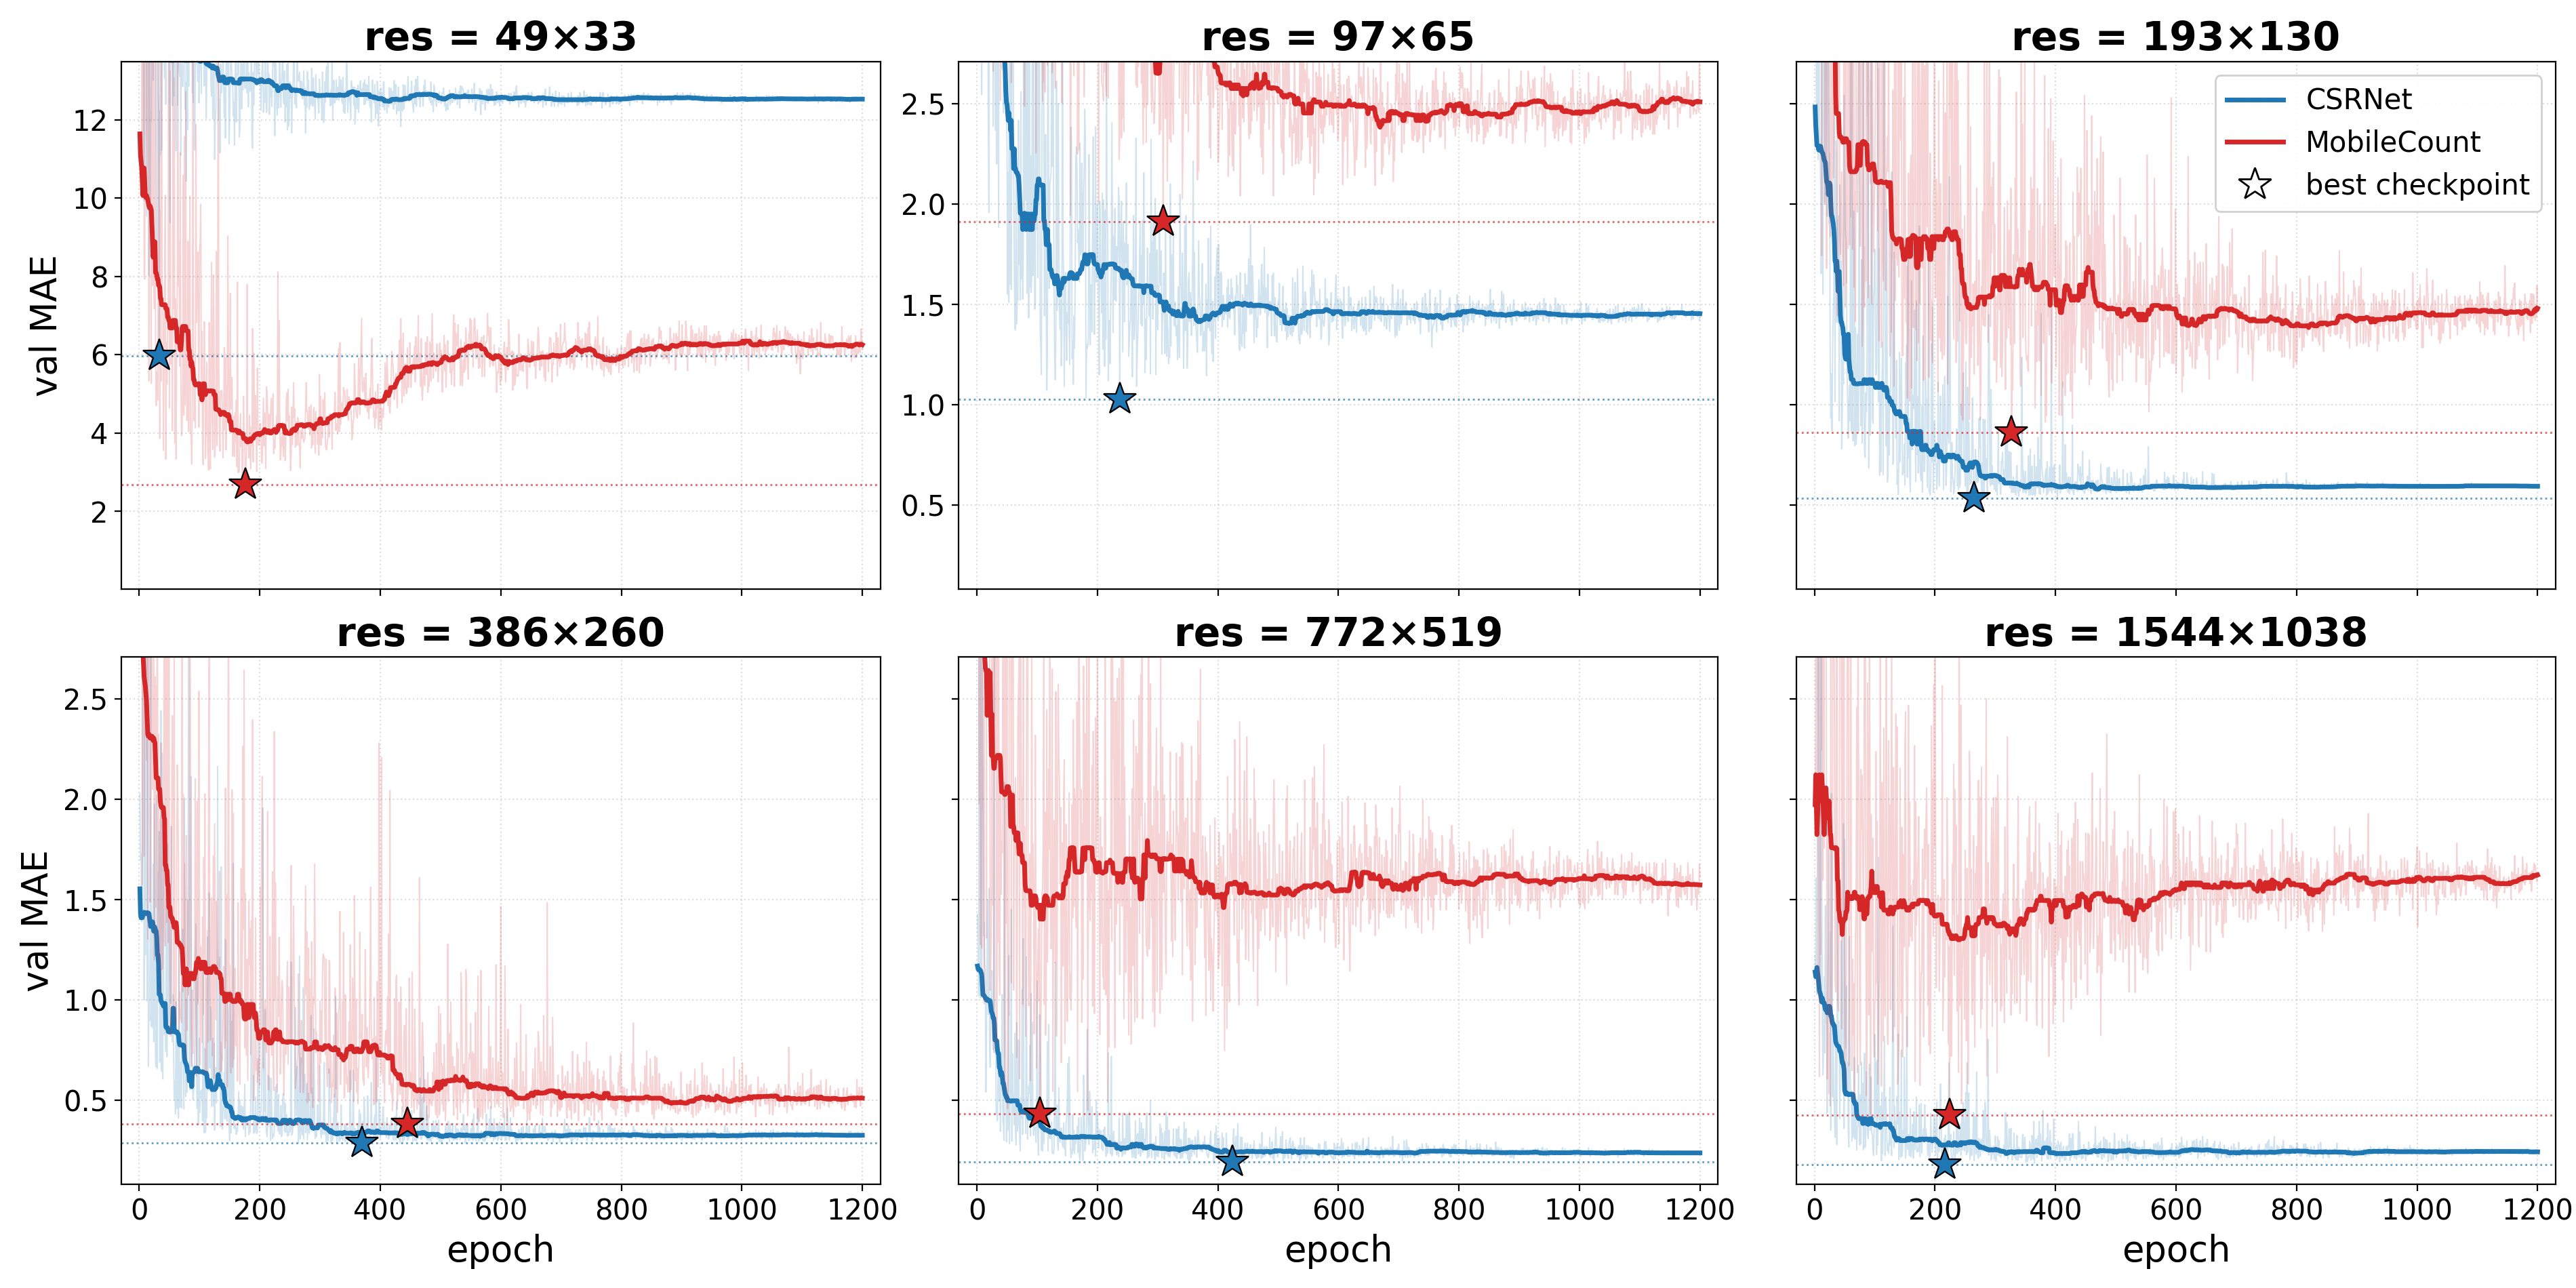
\includegraphics[width=0.75\linewidth]{images/mae_curves_by_resolution_thesis_2x3.png}
        \caption{Validation MAE over training for the tuned configurations across all six resolution variants. Curves are truncated at epoch $1200$ for legibility; no run changes materially during the final $300$ epochs.}
    \label{fig:res_learning_curves}
\end{figure*}

\subsection{Peak Inference Memory}
\begin{figure}
    \centering
    
\includegraphics[width=\linewidth]{images/mae_vs_memory.png}
    \caption{Accuracy--memory frontier: test MAE against peak batch-1
    inference memory for all twelve network~$\times$~resolution cells
    (log--log). Labels give the input resolution; lower-left is
    better.}
        \label{fig:acc_vs_mem}
\end{figure}

Figure~\ref{fig:acc_vs_mem} relates each cell's test MAE to its measured peak
inference memory. MobileCount occupies the low-memory regime throughout.
Across the three smallest resolutions, peak memory is nearly constant —
$80$--$89$\,MB for CSRNet and $13$--$16$\,MB for MobileCount — because it is
dominated by the resident model weights ($63.8$\,MB for CSRNet's $16.26$\,M
parameters versus $13.1$\,MB for MobileCount's $3.40$\,M, in $32$-bit
precision). From $386\times260$ onward the intermediate activations become the
dominant contributor, and peak memory grows roughly in proportion to the input
pixel count, reaching $1649$\,MB for CSRNet and $204$\,MB for MobileCount at
the largest resolution.

In Pareto terms, MobileCount dominates CSRNet over most of the operating
range: down to its own best test MAE of $0.361$, every accuracy level it
reaches costs a fraction of CSRNet's memory. At the shared tuning resolution
of $386\times260$, MobileCount is simultaneously more accurate ($0.433$ vs.\
$0.470$) and $6.4\times$ cheaper in memory ($26$ vs.\ $165$\,MB). CSRNet
becomes Pareto-optimal only beyond the lightweight network's accuracy ceiling:
its $772\times519$ and $1544\times1038$ configurations reach MAEs of $0.289$
and $0.233$ — below MobileCount's best result — at $460$\,MB and $1.6$\,GB of
peak memory respectively.

\section{Discussion}\label{sec:discussion}
\subsection{Implications for Edge Deployment}
To ground these figures in the deployment scenario motivating this work,
consider the NVIDIA Jetson Nano, a representative embedded module for on-site
inference. The Nano provides $4$\,GB of LPDDR4 memory shared between CPU and
GPU~\cite{nvidia2024jetsonnano}, so the budget effectively available to a
network at inference time is well below the nominal capacity once the
operating system, GPU driver, and CUDA runtime are resident. Against this
budget, MobileCount's $26$\,MB peak at $386\times260$ is negligible; CSRNet's
$460$\,MB at $772\times519$ already claims a substantial fraction of the
usable headroom, and its $1.6$\,GB at $1544\times1038$ approaches the
practical limit of the device.

This resolves the question posed in Section~\ref{sec:intro}: the ranking of
the ``smart but heavy'' and ``simple but light'' strategies is not fixed but
conditional on the accuracy requirement. If a counting error of roughly one
percent of the mean count (${\approx}0.4$--$0.5$ larvae) suffices — a
plausible tolerance for feeding and harvesting decisions — the lightweight
model at a moderate resolution meets it with two orders of magnitude of
memory headroom, and nothing about the heavy model's accuracy advantage
justifies its cost. Only when errors below the lightweight network's observed
ceiling of ${\approx}0.36$ are required does the heavyweight model become the
only option, and even its most accurate configuration still fits — barely —
within the device's budget.

\subsection{Limitations}
Four limitations qualify these conclusions.

\paragraph{Hyperparameters transported from a single resolution}
The largest limitation is that hyperparameters were optimised strictly at
$386\times260$ and applied unchanged across all resolutions. MobileCount's
saturation is confounded by this choice: its hyperparameters were selected at
the precise resolution where its performance peaks, and
Section~\ref{sec:results} shows its high-resolution runs failing through
optimisation instability rather than exhausted capacity. This tempers the
headline trade-off. CSRNet's Pareto-optimality at the high-accuracy end rests
on MobileCount's ceiling; had MobileCount trained stably at
$772\times519$ and $1544\times1038$ and continued its mid-range trajectory,
it might have matched the heavier network's accuracy at a tenth of the memory,
making it the better choice outright. Per-resolution retuning — at minimum of
the learning rate — is needed to close this question.

\paragraph{Deployment budget estimated, not measured}
The Jetson Nano analysis compares desktop-GPU allocator measurements against
the module's nominal capacity; how much of the $4$\,GB remains once the
operating system, driver, and CUDA context are resident was not measured, and
a different inference runtime may shift the absolute footprints. The relative
ordering of the twelve configurations is unaffected, but validating the
deployment claim by running the trained models on the actual hardware is the
natural next step.

\paragraph{Single random seed}
All results rest on a single random seed ($3035$), so seed-dependent noise
propagates through every selection made during tuning and into the final
comparison. Three-seed repeats run during earlier stages of tuning give a
sense of scale: best validation MAE varied by roughly $\pm0.01$ under AdamW
configurations and by up to $\pm0.05$ for MobileCount under Adam. Differences
of that order — such as MobileCount's test MAEs across its three largest
resolutions — should not be interpreted; the conclusions drawn here rest on
gaps an order of magnitude larger (CSRNet's monotonic gains, the
optimiser-grid margins, and the memory separation between the two networks).
Replicating the main grid over multiple seeds would make the smaller margins
interpretable as well.

\paragraph{Transfer to production imagery}
TenebrioVision was captured under fixed viewpoint, illumination, and
background conditions, and its authors report that models trained on it
degraded on real farm imagery, which they countered with targeted
augmentation~\cite{Papadopoulos2024TenebrioVision}. That augmentation recipe
(flips, rotation, per-channel radiometric jitter, and sparse noise) was
implemented and evaluated here as well: added to the tuned configurations at
$386\times260$, it left CSRNet slightly better ($0.288 \rightarrow 0.243$
validation MAE) but made MobileCount markedly worse
($0.385 \rightarrow 0.539$). Since no farm imagery is available in this study,
whether these augmentations would buy robustness where it matters cannot be
tested — only that their cost on in-distribution data differs sharply between
a pretrained and a from-scratch network. Evaluating the trained models on
production imagery remains future work.

\section{Conclusion}
This thesis compared two strategies for density-based counting of
\textit{Tenebrio molitor} larvae under edge-hardware memory constraints: a
heavyweight network on downscaled inputs versus a lightweight network with
headroom for full-resolution inputs. Both networks proved remarkably robust to
downscaling, counting to within one larva of the ground truth at a sixteenth
of the native pixel count. Beyond that, the strategies separate: CSRNet
converts every additional pixel into accuracy, down to a test MAE of $0.233$
at $1.6$\,GB of peak inference memory, while MobileCount plateaus near $0.36$
at just $204$\,MB — and holds the accuracy--memory Pareto frontier everywhere
above that ceiling. For the counting tolerances plausible in mealworm farming,
the answer to the research question is therefore that input fidelity beats
architectural complexity: the lightweight model fed adequately sized images is
the clear deployment choice, and the heavyweight model is justified only when
sub-$0.3$-larva accuracy is a hard requirement. Training diagnostics suggest
even that niche may be contestable, as the lightweight network's ceiling
reflects optimisation instability under transported hyperparameters rather
than a demonstrated capacity limit. On-device validation, per-resolution
retuning, multi-seed replication, and evaluation on production farm imagery
are the natural extensions of this work.

\bibliographystyle{IEEEtran}
\bibliography{references}


\end{document}
